\documentclass[aspectratio=169,11pt]{beamer}
\usepackage{amsmath,amssymb,booktabs,graphicx,tikz,pgfplots}
\pgfplotsset{compat=1.18}
\usetheme{Boadilla}
\useoutertheme[subsection=false]{miniframes}
\definecolor{ugared}{HTML}{BA0C2F}
\definecolor{ugablack}{HTML}{000000}
\setbeamercolor{structure}{fg=ugared}
\setbeamercolor{alerted text}{fg=ugared}
\setbeamercolor{normal text}{fg=ugablack,bg=white}
\setbeamercolor{frametitle}{fg=white,bg=ugared}
\setbeamercolor{title}{fg=white,bg=ugared}
\setbeamercolor{block title}{fg=white,bg=ugablack}
\setbeamercolor{block body}{fg=ugablack,bg=ugared!5!white}
\setbeamercolor{section in toc}{fg=ugared}
\setbeamercolor{palette primary}{fg=white,bg=ugared}
\setbeamercolor{palette secondary}{fg=white,bg=ugablack}
\setbeamercolor{section in head/foot}{fg=ugared,bg=white}
\setbeamercolor{mini frame}{fg=ugared,bg=white}
\setbeamercolor{upper separation line head}{bg=white}
\setbeamercolor{lower separation line head}{bg=ugared}
\setbeamerfont{section in head/foot}{size=\scriptsize}
\setbeamertemplate{mini frames}[default]
\setbeamertemplate{navigation symbols}{}
\setbeamertemplate{footline}{\hfill\insertshorttitle\quad|\quad\insertframenumber\hspace{5mm}\vspace{3mm}}
\setbeamertemplate{itemize items}[circle]
\setbeamerfont{frametitle}{size=\Large}
\setlength{\parskip}{6pt}
\graphicspath{{assets/}}
\title[Dynamic Optimal Pricing]{Dynamic Optimal Pricing with Love of Variety}
\author{Tate Mason}
\date{MacrIOT 2026}
% Speaker notes are embedded but hidden. To print notes, add:
% \\setbeameroption{show notes}
\begin{document}
\begin{frame}[plain]
\titlepage
\note{Introduce the research question: what can purchase histories tell firms about preferences for switching?}
\end{frame}

\section{Introduction}
\begin{frame}{Introduction}
\begin{block}{Research question}How do firms augment their optimal pricing strategy when love of variety is present?\end{block}
\begin{itemize}
\item Repeated consumption may reduce the appeal of a product.
\item Purchase histories can reveal when a consumer is ready to switch.
\item Retailers can leverage that information to optimally price according to the distribution of consumers.
  \begin{itemize}
    \item Dynamic price setting
    \item Targeting
  \end{itemize}
\end{itemize}
\note{Use the example of someone who likes berry yogurt but wants something different after repeated purchases. Distinguish a stable taste from fatigue.}
\end{frame}

\begin{frame}{Motivation}
\begin{block}{Motivation}
\begin{itemize}
\item \textbf{Pricing:} knowing switching types raises per-unit profits by up to about 2 cents in the reported normalization.
\item \textbf{Demand:} flavor preferences change little when fatigue is included; some fatigue parameters are weakly identified.
\end{itemize}
\end{block}
\begin{block}{Contribution}
\begin{itemize}
  \item Estimate distribution of LOV types 
  \begin{itemize}
    \item Lattin (1987), Chintagunta (1996), Dub\'e (2003)
  \end{itemize}
  \item Connect switching preferences and state dependence to the information a retailer uses for pricing
  \begin{itemize}
    \item Dub\'e and Misra (2023), Moorthy and Tehrani (2023), Karle and Reisinger (2024)
  \end{itemize}
\end{itemize}
\end{block}
\note{Explain upfront that the empirical demand model and toy supply model are separate exercises.

Position relative to attribute satiation in McAlister and Lattin, brand dynamics in Chintagunta, and personalized pricing in Dube and Misra. References are in the backup slides.}
\end{frame}

\section{Pricing Model}
\begin{frame}{Pricing Model}
\begin{itemize}
\item Purchase histories can reveal preferences for switching between products.
\item The supply exercise asks how a retailer would price if switching types were known or inferred.
  \begin{itemize}
    \item How do they dynamically price?
    \item How does the firm price discriminate?
  \end{itemize}
\item Two products, two types, two periods.
\end{itemize}
\note{Introduce the illustrative supply exercise before turning to demand. Supply uses a positive reward for switching, whereas demand uses a negative coefficient on a fatigue stock.}
\end{frame}

\begin{frame}{Supply model}
\begin{block}{Consumer's value from choosing product $j$}
\[
V_{rjt}=\underbrace{\beta_{0j}}_{\text{baseline preferences}}
+\underbrace{\gamma_r\mathbf{1}\{j\ne j_{t-1}\}}_{\text{love of variety}}
+\underbrace{\alpha p_{rjt}}_{\text{price effect}},
\qquad r\in\{H,L\}.
\]
\end{block}
\begin{itemize}
\item $V_{rjt}$ is the deterministic utility of product $j$ for a type-$r$ consumer at time $t$.
\item Switching from the previously chosen product $j_{t-1}$ adds $\gamma_r$; choosing it again adds no switching reward.
\item High types value switching more: $\gamma_H>\gamma_L$. A higher price lowers utility ($\alpha<0$).
\item Consumers choose the highest utility after logit choice shocks; the outside option allows no purchase.
\end{itemize}
\note{Explain the equation from the consumer's perspective: baseline product appeal, a reward for choosing a different product from last period, and a negative price effect. V is deterministic current-period utility, not a forward-looking consumer Bellman value. Adding independent type-I extreme-value shocks gives logit choice probabilities including an outside option. The retailer uses these probabilities in its pricing problem. Use s for a probability or share, not a sum of probabilities over consumers. Population size multiplies per-consumer profits.}
\end{frame}

\begin{frame}{Perfect information}
\begin{block}{Perfect information}The retailer conditions prices on known type and observed purchase history.\end{block}
$W_r(j)$ is the retailer\textquotesingle s optimal period-two profit per consumer, given type $r$ and first-period choice $j$.
\[
W_r(j)=\max_{\mathbf p_2(j)}\sum_k s_{rk2}(j)\bigl(p_{rk2}(j)-c_k\bigr),
\]
\[
\Pi^{\rm full}=\sum_r N_r\sum_j s_{rj1}
\left[p_{rj1}-c_j+\delta W_r(j)\right].
\]
A lower price today can move a consumer into a more profitable state tomorrow.
\note{Here j includes all first-period outcomes, including no purchase, with zero outside margin and an explicitly defined continuation state. This compact objective avoids reproducing the draft long first-order conditions, whose outside-option treatment is ambiguous.}
\end{frame}

\begin{frame}{Learning}
\[
q=\Pr(r=H),\qquad \tilde s_{j1}=q s_{Hj1}+(1-q)s_{Lj1},
\]
\[
q_2(j)=\Pr(H\mid j)=\frac{q s_{Hj1}}{q s_{Hj1}+(1-q)s_{Lj1}}.
\]
\begin{itemize}\item Period-one prices are common across unobserved types.\item Period-two prices depend on observed purchase history.\item A choice relatively more likely for high types raises the posterior.\end{itemize}
\note{A posterior above the prior conditional on a purchase is not inherently biased or an overestimate. Bayes plausibility requires averaging over all outcomes, including no purchase. The simulation table reports only the inside-good posteriors.}
\end{frame}

\begin{frame}{Limited information}
\[
\Pi^{\rm limited}=N\sum_j\tilde s_{j1}(\mathbf p_1)
\left[p_{j1}-c_j+\delta W\bigl(j,q_2(j;\mathbf p_1)\bigr)\right].
\]
\begin{enumerate}\item Current margin versus current demand.\item How purchases change future consumption states.\item How purchases reveal switching type.\end{enumerate}
\begin{block}{Mechanism}Prices influence both allocation and the informativeness of observed choices.\end{block}
\note{This objective expresses the mechanism without relying on the source algebra for the learning derivative. The sign of a price response is not universal; focus on the reported simulation. Include outside histories when implementing the objective.}
\end{frame}



\begin{frame}[label=supply-results]{Supply results}
\begin{columns}\begin{column}{.58\textwidth}
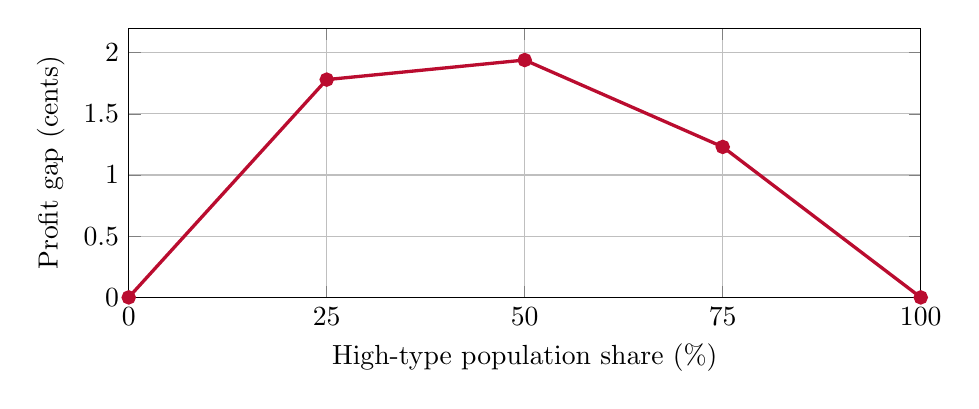
\begin{tikzpicture}\begin{axis}[width=.96\linewidth,height=5cm,xlabel={High-type population share (\%)},ylabel={Profit gap (cents)},xmin=0,xmax=100,ymin=0,ymax=2.2,xtick={0,25,50,75,100},grid=major]
\addplot[color=ugared,very thick,mark=*] coordinates {(0,0)(25,1.78)(50,1.94)(75,1.23)(100,0)};
\end{axis}\end{tikzpicture}
\end{column}\begin{column}{.38\textwidth}
\begin{block}{Reported value of information}Full-information profit minus limited-information profit.\end{block}
Largest gap: \alert{1.94 cents} at a 50/50 type mix.
\end{column}\end{columns}
\note{Chart is redrawn from the value-of-information column, not recalculated from rounded profit columns. Retain the reported normalization; the draft calls it per unit but the objective is written per consumer over two periods. This requires clarification before quantitative policy use.}
\par\smallskip
\hyperlink{supply-parameters}{\beamerbutton{Simulation parameters}}
\end{frame}

\begin{frame}{Pricing results}
\centering
{\small Information Structure, Optimal Pricing, and Value of Information Across Population Mixes\par}
\vspace{5mm}
\renewcommand{\arraystretch}{1.25} % Adds comfortable vertical breathing room
\resizebox{\textwidth}{!}{% Fits perfectly to text margins without crowding
\begin{tabular}{l r r r r r r r}
\toprule
\textbf{Population Mix} & \multicolumn{2}{c}{\textbf{Imperfect Price ($P_1$)}} & \multicolumn{2}{c}{\textbf{Posterior Beliefs}} & \textbf{Imperfect} & \textbf{Perfect} & \textbf{Value of} \\
& \textbf{Good 1} & \textbf{Good 2} & \textbf{G1} & \textbf{G2} & \textbf{Profit} & \textbf{Profit} & \textbf{Info} \\
\midrule
100\% LOW           & 2.0633 & 1.8646 & 0.0000 & 0.0000 & 0.6031 & 0.6031 & -0.0000 \\
25\% HIGH, 75\% LOW & 2.1847 & 1.9944 & 0.3727 & 0.3641 & 0.7820 & 0.7999 &  0.0178 \\
50\% HIGH, 50\% LOW & 2.2819 & 2.1049 & 0.6510 & 0.6448 & 0.9773 & 0.9966 &  0.0194 \\
75\% HIGH, 25\% LOW & 2.3542 & 2.1887 & 0.8528 & 0.8504 & 1.1811 & 1.1934 &  0.0123 \\
100\% HIGH         & 2.4067 & 2.2494 & 1.0000 & 1.0000 & 1.3902 & 1.3902 &  0.0000 \\
\bottomrule
\end{tabular}%
}

\note{Table from the full paper with the redundant percentage-high and percentage-low columns removed; population mixes, prices, posterior beliefs, profits, and reported information values are retained.}
\end{frame}









\section{Data}
\begin{frame}{Data}
\begin{itemize}
\item Nielsen HomeScan and MarketScan, 2022--2024.
\item Eight markets: Atlanta, Chicago, Denver, Houston, Des Moines, Phoenix, Philadelphia, San Diego.
\item Single-person households reduce ambiguity about whose tastes drive purchases.
\item Single-serving yogurt offers flavor variation and limited storability.
\end{itemize}
\note{Single-person households help with interpretation but do not eliminate measurement issues or purchases for others.}
\end{frame}

\begin{frame}{Sample}
\centering
\begin{tabular}{lrr}\toprule
 & Full sample & Estimation sample\\\midrule
Households & 5,408 & 998\\
Mean store trips / household & 308.15 & 400.05\\
Mean observed yogurt choice weeks & --- & 3.91\\
Coupon / deal purchase rate & 26.52\% & 23.10\%\\
Mean weekly yogurt units (purchasers) & --- & 8.44\\\bottomrule
\end{tabular}
\vspace{4mm}
\begin{block}{Implication}The panel contains limited yogurt history for many households.\end{block}
\note{Report these as the draft table statistics. Do not infer a trip frequency from the eight-week observation description; the aggregation needs reconciliation before doing so.}
\end{frame}

\begin{frame}{Flavor groups}
\begin{itemize}
\item \textbf{Berry:} berry-labeled flavors plus cherry.
\item \textbf{Plain:} a separate category.
\item \textbf{Other:} all remaining flavors.
\item \textbf{Outside option:} no yogurt purchase.
\end{itemize}\begin{block}{Tradeoff}Aggregation makes estimation tractable but hides switching within a flavor group.\end{block}
\note{Emphasize that changing from vanilla to peach is invisible in the other category. This can suppress measured variety seeking.}
\end{frame}

\begin{frame}{Flavor concentration}
\centering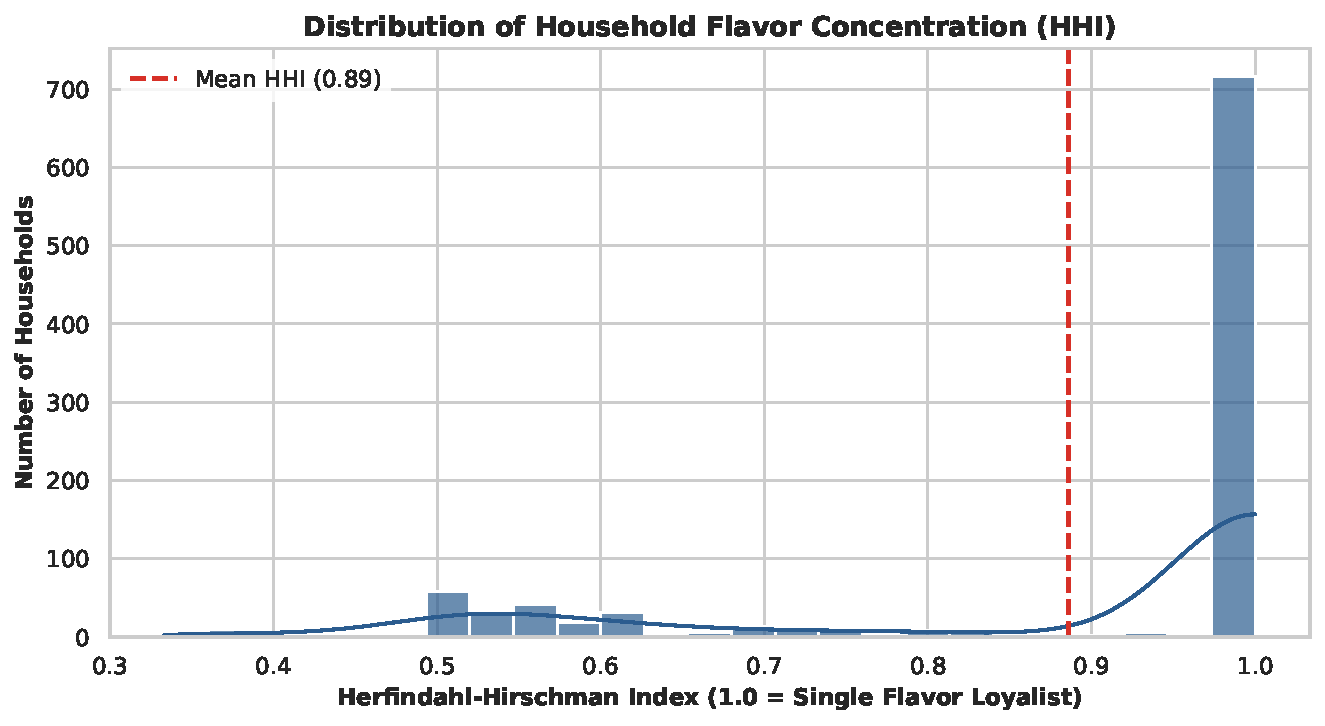
\includegraphics[height=.67\textheight,width=.94\textwidth,keepaspectratio]{fig1_flavor_hhi_distribution.pdf}
\note{The draft reports that over 70 percent are nearly loyal to one group. Concentration is at the aggregate flavor level, not necessarily at the individual flavor or brand level.}
\end{frame}

\begin{frame}{Flavor shares}
\centering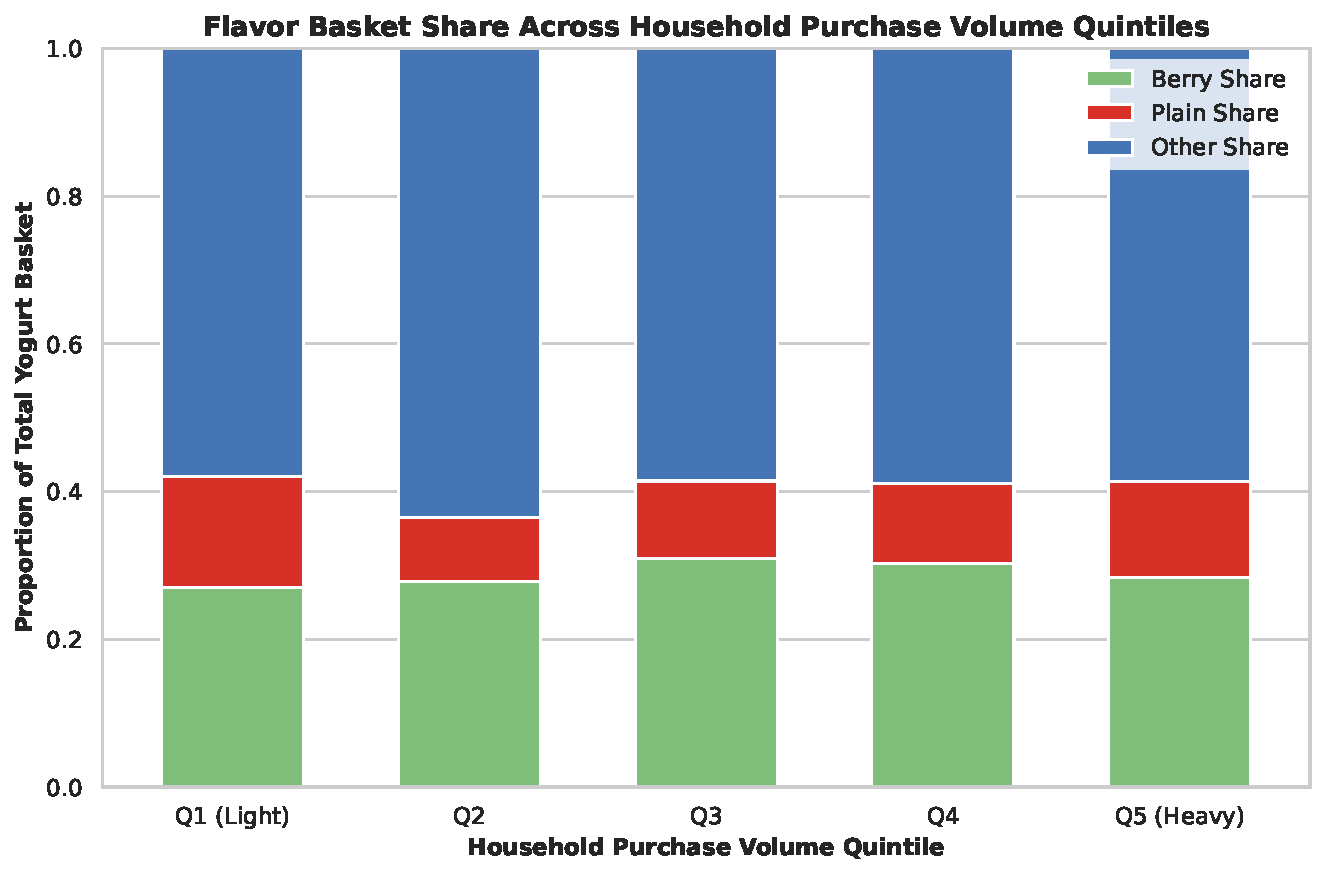
\includegraphics[height=.67\textheight,width=.94\textwidth,keepaspectratio]{fig2_basket_share_by_volume.pdf}
\note{Other is around 60 percent across volume groups. Discuss how the uneven breadth of the categories affects interpretation.}
\end{frame}



\section{Empirical exercise}
\begin{frame}[label=demand-model]{Demand model}
\[
U_{ijt}=\underbrace{\beta_0+\beta_i'X_{jt}}_{\text{baseline tastes}}
+\underbrace{\gamma_i\Xi_{ijt}}_{\text{history state}}
+\underbrace{\alpha p_{jt}}_{\text{price}}+\varepsilon_{ijt}.
\]

  \[
  \text{s.t.} \ 
  \Xi_{ijt} = \lambda\sum_{s=1}^8\delta^{t-s}\Xi_{ij,t-s} + (1-\lambda)\sum_{k\ne j}\rho_kX_{k,t-1}
\]
\begin{itemize}
\item Inside choices: berry, plain, other; outside utility normalized to zero.
\item $\Xi_{ijt}$ summarizes prior consumption and switching.
\item Negative fatigue coefficients reduce utility as the history index rises.
\end{itemize}
\note{The next slides define the full manuscript-style history index and show its update. Distinguish the intended fatigue motivation from the cross-flavor construction. Demand history coefficients and supply switching rewards have different sign conventions.}
\par\smallskip
\hyperlink{simulation-procedure}{\beamerbutton{Simulation procedure}}\quad
\hyperlink{simulation-results}{\beamerbutton{Simulation results}}\quad
\hyperlink{utility-specification}{\beamerbutton{Utility specification}}
\end{frame}

\begin{frame}{Identification}
\begin{itemize}
\item \textbf{Stable tastes:} persistent differences in flavor choices.
\item \textbf{Fatigue:} changes in choices associated with a household\textquotesingle s own history.
\item \textbf{Challenge:} heterogeneity, prices, and unobserved shocks can also generate switching.
\item \textbf{Limited history and coarse groups} make the distinction difficult.
\end{itemize}
\note{A switching pattern alone does not identify fatigue. Discuss initial conditions, serially correlated shocks, and the amount of within-household variation required.}
\end{frame}
\begin{frame}{Price control function}
\[
p_{jmt}=a+b\underbrace{\bar p_{j,-m,t}}_{\text{other-market price}}
+\tau_t+\eta_{jmt},\qquad
\hat\eta_{jmt}=p_{jmt}-\hat p_{jmt}.
\]
\begin{enumerate}
\item Match household choices to flavor-specific prices and purchase histories.
\item Regress local prices on other-market prices and time controls.
\item Include the fitted residual in utility to account for endogenous prices.
\end{enumerate}
\begin{block}{Required exclusion}Other-market prices must shift local prices without sharing unobserved local demand shocks, conditional on the controls.\end{block}
\note{This is the Petrin--Train control-function approach used in the draft. First-stage coefficients are written explicitly. The draft does not provide instrument strength diagnostics and is inconsistent about the number of other markets.}
\end{frame}




\begin{frame}[label=specifications]{Specifications}
\centering
\begin{tabular}{lcc}\toprule
 & No fatigue & With fatigue\\\midrule
Standard logit & Fixed $\beta$; $\gamma=0$ & Fixed $\beta,\gamma$\\[2mm]
Random coefficient logit & Heterogeneous $\beta$; $\gamma=0$ & Heterogeneous $\beta,\gamma$\\\bottomrule
\end{tabular}
\begin{itemize}
\item Price and the control-function residual enter all four specifications.
\item Compare baseline flavor tastes and price effects across columns.
\item Assess fatigue means and dispersion separately from optimizer convergence.
\item Identification depends on within-household history variation, valid price instruments, and the treatment of initial histories.
\end{itemize}
\note{The distribution and numerical integration details should be checked against the estimation implementation before presenting this likelihood as a verified account of the code. National common demand shocks can threaten the price instrument. Results follow immediately.}
\par\smallskip
\hyperlink{panel-likelihood}{\beamerbutton{Panel likelihood}}
\end{frame}


\begin{frame}{Demand estimates}
\centering\small
\begin{tabular}{lrrrr}\toprule
& \multicolumn{2}{c}{Standard logit} & \multicolumn{2}{c}{Random coefficients}\\
& No Variety & Variety & No Variety & Variety\\\midrule
Berry preference & $-.7635$ & $-.7576$ & $-.7632$ & $-.7489$\\
Plain preference & $-1.3899$ & $-1.3897$ & $-1.3930$ & $-1.3956$\\
Price & $-.9836$ & $-.9821$ & $-.9836$ & $-.9804$\\
Control function & $.1670$ & $.1667$ & $.1654$ & $.1662$\\\bottomrule\end{tabular}
  \begin{itemize}
    \item All estimates relative to other flavors and the outside option
  \end{itemize}

\begin{block}{Main empirical result}The largest baseline flavor change is about 1.9\% for berry in the random coefficient model.\end{block}
\note{Flavor coefficients are relative to other; the intercept locates inside utility relative to the outside option. The largest percentage change is in magnitude. These estimates are reported as significant in the source tables.}
\end{frame}

\begin{frame}{LOV coefficients}
\centering
\begin{tabular}{lrr}\toprule
 & Standard logit & Random coefficients\\\midrule
Berry LOV & $-.7262$ & $-7.2030$\\
Standard error & $(.1485)$ & $(1.5424)$\\[2mm]
Plain LOV & $-.0351$ & $-.0555$\\
Standard error & $(.1009)$ & $(.1032)$\\\bottomrule\end{tabular}
\begin{itemize}\item Berry has a negative estimated history coefficient.\item Plain is not statistically distinguishable from zero.\item Large changes across specifications warrant caution.\end{itemize}
\note{A negative coefficient means history lowers utility under the fatigue index interpretation. Do not confuse a significant mean with precise identification of its heterogeneity.}
\end{frame}

\begin{frame}{Heterogeneity}
\begin{columns}[T]\begin{column}{.5\textwidth}
\small\begin{tabular}{lrr}\toprule
Random coefficient SD & Estimate & SE\\\midrule
$\beta_{\rm berry}$ & 1.0513 & .0916\\
$\beta_{\rm plain}$ & 1.0513 & .1492\\
$\gamma_{\rm berry}$ & 148.4132 & 155.3868\\
$\gamma_{\rm plain}$ & 1.0513 & .1641\\\bottomrule\end{tabular}
\end{column}\begin{column}{.46\textwidth}
\begin{block}{Diagnostic}The berry LOV dispersion is extremely large and imprecisely estimated.\end{block}
Optimization success alone does not establish reliable identification.
\end{column}\end{columns}
\note{These values contradict the prose claim of little taste heterogeneity. The repeated standard deviations and large berry value should be audited against estimation code. Treat them as reported estimates, not validated structural distributions.}
\end{frame}

\begin{frame}{Implied WTP}
\centering\begin{tabular}{lrr}\toprule
Magnitude in dollars & Standard & Random coefficients\\\midrule
Berry preference & .77 & .76\\
Plain preference & 1.42 & 1.42\\
Berry fatigue & .74 & 7.35\\
Plain fatigue & .04 & .06\\\bottomrule\end{tabular}
\[
\text{Implied WTP}=\frac{|\text{utility coefficient}|}{|\alpha|}.
\]
\begin{block}{Interpretation}The large \$7.35 number belongs to berry LOV and is sensitive to the specification.\end{block}
\note{These are magnitudes, not positive willingness to pay for a disliked flavor. The fatigue ratio is per unit of the history index, not automatically the discount needed after one repeated purchase. Avoid treating the large mixed-logit ratio as a precise policy target.}
\end{frame}

\section{Conclusion}
\begin{frame}{Conclusion}
\begin{itemize}
\item Restricting type information can reduce retailer profits in this model.
\item The loss is greatest when the population contains both switching types.
\item Attribute fatigue lowers consumer utility
\item Difficult to disentangle preferences from love of variety
\end{itemize}
\note{Distinguish the illustrated cost of an information constraint from a causal estimate of an actual regulation. A policy conclusion needs consumer welfare, collection costs, and an explicit policy mapping.}
\end{frame}

\appendix
\setbeamertemplate{headline}{}

\begin{frame}[noframenumbering,label=supply-parameters]{Simulation parameters}
\centering\begin{tabular}{ll}\toprule
Baseline product utilities & $(2.2,2.0)$\\
Switching utility $(\gamma_H,\gamma_L)$ & $(2.0,0.1)$\\
Price coefficient $\alpha$ & $-1.5$\\
Discount factor $\delta$ & $0.95$\\
Unit costs $(c_1,c_2)$ & $(1.2,1.0)$\\
Initial product-state weights & $(0.5,0.5)$\\
Price bounds & $[\$1,\$8]$\\\bottomrule\end{tabular}
\begin{block}{Comparison}Vary the high-type population share under full and limited information.\end{block}
\note{No empirical calibration is claimed. The source does not fully document the profit denominator or the initial-history implementation; preserve the table values and label the normalization cautiously.}
\par\smallskip
\hyperlink{supply-results}{\beamerreturnbutton{Supply results}}
\end{frame}

\begin{frame}[noframenumbering,label=simulation-procedure]{Simulation procedure}
\small
\begin{tabular}{ll}\toprule
Simulation design & Assigned value\\\midrule
Replications / evaluation periods / burn-in & $1{,}000\;/\;100\;/\;5$\\
Product attributes / baseline taste & $X_j\in\{1,2,3,4,5\}\;;\;\beta=2$\\
Variety grid / choice shocks & $\gamma\in\{0,3,6,9\}\;;\;\varepsilon_{jt}\sim\mathrm{T1EV}$\\\bottomrule
\end{tabular}
\begin{enumerate}
\item For each $\gamma$, initialize consumption histories during burn-in.
\item At each evaluation date, combine baseline attribute utility with the history-dependent distance reward and a choice shock.
\item Record the selected product, update its consumption history, and repeat.
\item Summarize choice probabilities across the simulated runs.
\end{enumerate}
\textbf{Purpose:} show how variety changes choices in a controlled setting.
\note{The procedure summarizes the simulation described in the manuscript. Its distance-based mechanism differs from the empirical flavor-fatigue index. Simulation code is not re-estimated here.}
\par\smallskip
\hyperlink{simulation-results}{\beamerbutton{Simulation results}}\quad \hyperlink{demand-model}{\beamerreturnbutton{Demand model}}
\end{frame}

\begin{frame}[noframenumbering,label=simulation-results]{Simulation results}
\centering
\begin{tabular}{lrrrr}\toprule
 & $\gamma=0$ & $\gamma=3$ & $\gamma=6$ & $\gamma=9$\\\midrule
Product 1 ($X=1$) & .0016 & .1352 & .3321 & .3973\\
Product 2 ($X=2$) & .0084 & .1325 & .0541 & .0084\\
Product 3 ($X=3$) & .0437 & .0844 & .0026 & .0000\\
Product 4 ($X=4$) & .1934 & .0553 & .0023 & .0002\\
Product 5 ($X=5$) & .7529 & .5926 & .6089 & .5941\\\bottomrule
\end{tabular}
\begin{block}{Interpretation}Without variety, the highest-attribute product dominates. With stronger variety, choices concentrate at the endpoints.\end{block}
\small This motivates modeling history; it does not establish identification in the yogurt panel.
\note{Walk through product 1 and product 5, then the disappearance of the middle products. Values are taken directly from the source table.}
\par\smallskip
\hyperlink{simulation-procedure}{\beamerbutton{Simulation procedure}}\quad \hyperlink{demand-model}{\beamerreturnbutton{Demand model}}
\end{frame}

\begin{frame}[noframenumbering,label=utility-specification]{Utility specification}
\small
For $j\in\{B,P,O\}$ (berry, plain, other), let $D_j^f=\mathbf1\{j=f\}$:
\[
\begin{aligned}
U_{ijt}&=V_{ijt}+\varepsilon_{ijt},\\
V_{ijt}&=\beta_0+\beta_i^B D_j^B+\beta_i^P D_j^P\\
&\quad+\gamma_i^B D_j^B\Xi_{ijt}
+\gamma_i^P D_j^P\Xi_{ijt}
+\alpha p_{j,m(i),t}+\sigma\hat\eta_{j,m(i),t}.
\end{aligned}
\]
\begin{itemize}
\item Other flavor is the reference; outside deterministic utility is zero.
\item $\Xi_{ijt}$ summarizes own past consumption and alternative-flavor history.
\item History weight $\lambda=0.7$ and decay $\delta=0.9$ are fixed.
\item Random coefficients allow persistent household differences in tastes and fatigue.
\end{itemize}
\note{This expands the estimation formula using the flavor-specific parameters actually reported in the draft tables. The preceding slides define the manuscript-style history recursion using only past observed periods and explain its cross-flavor construction. The reference category normalizations match the reported tables.}
\par\smallskip
\hyperlink{demand-model}{\beamerreturnbutton{Demand model}}
\end{frame}

\begin{frame}[noframenumbering,label=panel-likelihood]{Panel likelihood}
\small
Conditional on household coefficients $b_i=(\beta_i^B,\beta_i^P,\gamma_i^B,\gamma_i^P)$:
\[
P_{ijt}(b_i)=\frac{e^{V_{ijt}(b_i)}}{1+\sum_{k\in\{B,P,O\}}e^{V_{ikt}(b_i)}},\qquad
P_{i0t}(b_i)=\frac{1}{1+\sum_k e^{V_{ikt}(b_i)}}.
\]
\[
L_i(b_i)=\prod_{t\in\mathcal T_i}\prod_{j\in\{0,B,P,O\}}
P_{ijt}(b_i)^{y_{ijt}},\qquad y_{ijt}=\mathbf1\{\text{observed choice is }j\}.
\]
\[
\boxed{\hat\theta=\arg\max_\theta\sum_i\log\!\left[\int L_i(b)\,dF(b;\theta)\right]}
\]
Simulation approximation: $\int L_i(b)dF(b;\theta)\approx R^{-1}\sum_{r=1}^R L_i(b_i^{(r)})$.

Maximize log-likelihood: $\ell(\theta)=\sum_{i,t,j}y_{ijt}\log P_{ijt}(\theta)$.
\note{Show that persistent household heterogeneity requires integrating the product over a household history, rather than multiplying separately integrated marginal probabilities. This is the full panel mixed-logit estimation target; the manuscript does not document the draw count or coefficient distribution, so neither is asserted here.}
\par\smallskip
\hyperlink{specifications}{\beamerreturnbutton{Specifications}}
\end{frame}

\begin{frame}[noframenumbering]{Discussion}
\begin{block}{Questions for discussion}
How can fatigue be distinguished from persistent unobserved tastes?\medskip

Which purchase histories are most informative about switching types?\medskip

What consumer-welfare evidence is needed to evaluate privacy restrictions?
\end{block}
\note{Optional discussion prompts.}
\end{frame}
\begin{frame}[noframenumbering]{Flavor shares over time}
\centering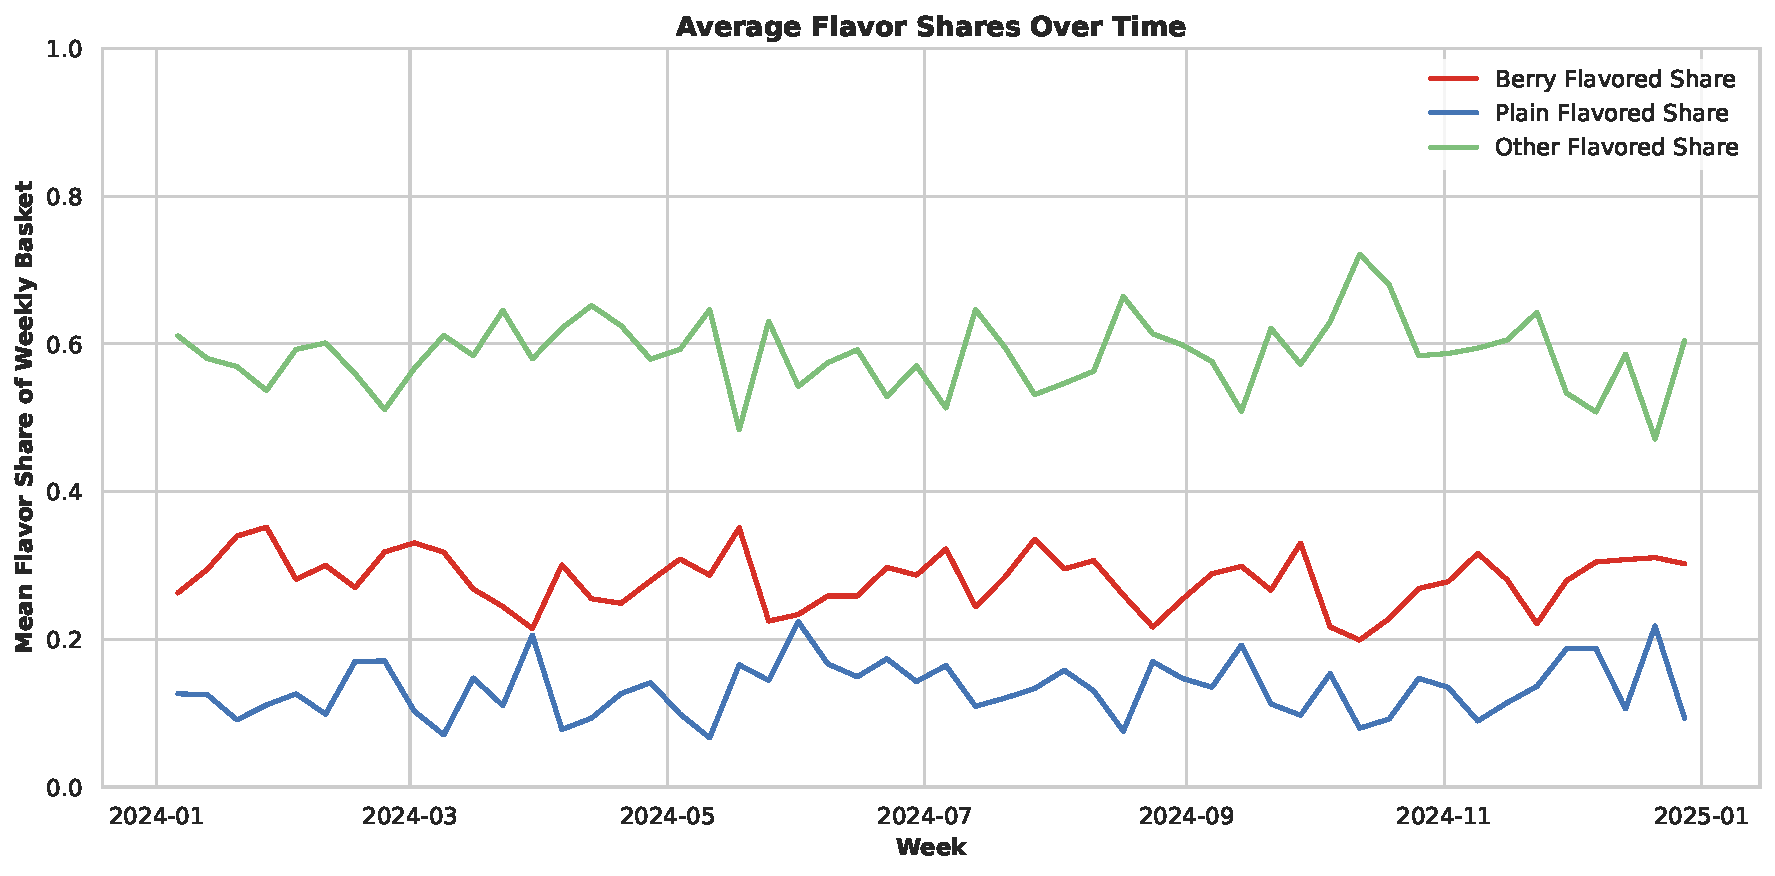
\includegraphics[height=.69\textheight,width=.95\textwidth,keepaspectratio]{fig3_flavor_share_timeseries.pdf}
\end{frame}
\begin{frame}[noframenumbering]{Marginal distributions}
\centering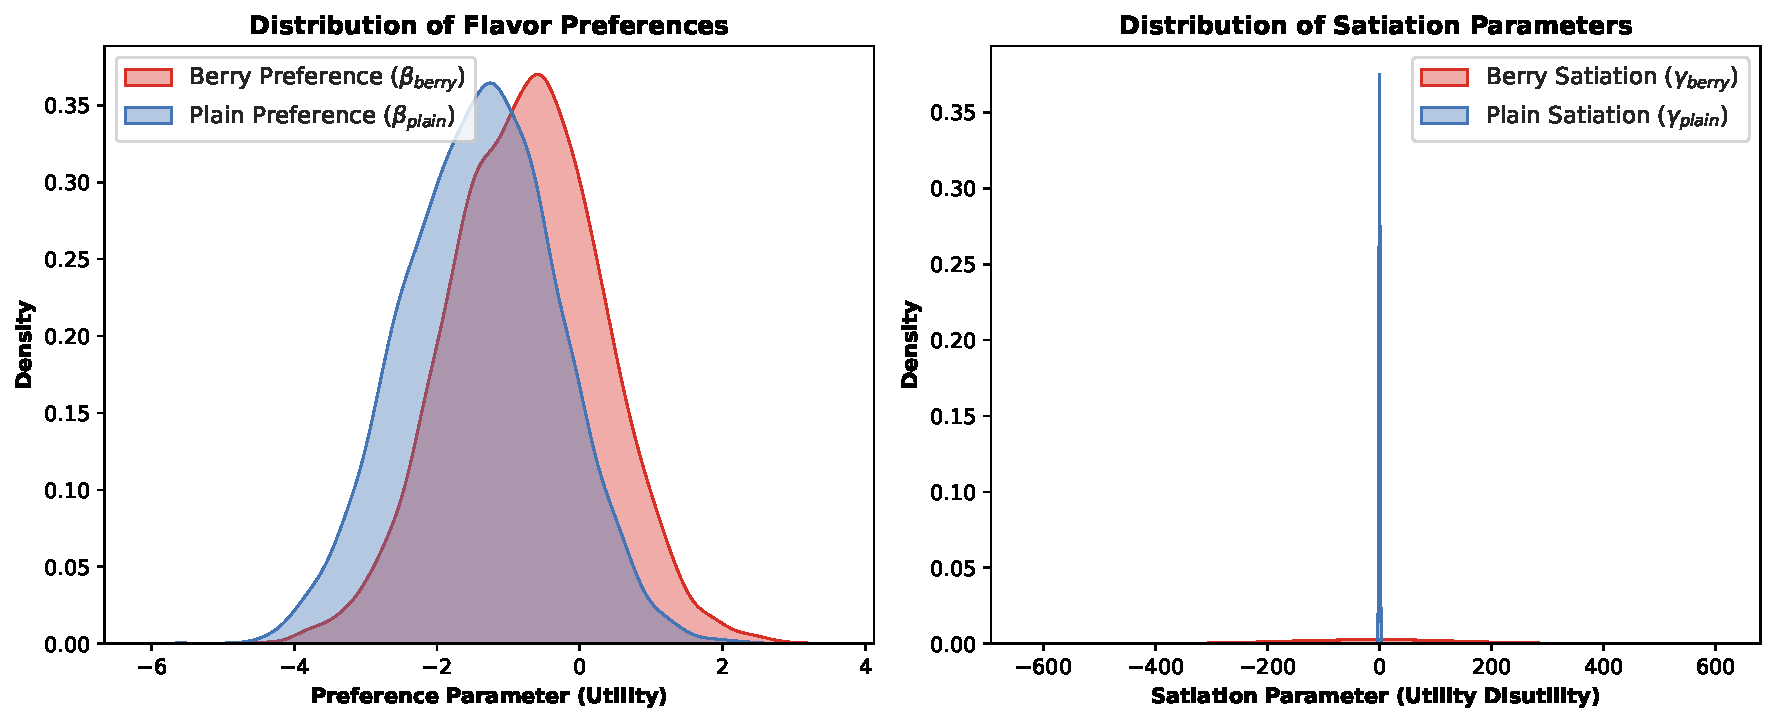
\includegraphics[height=.69\textheight,width=.95\textwidth,keepaspectratio]{fig4_marginal_type_distributions.pdf}
\end{frame}
\begin{frame}[noframenumbering]{Joint distributions}
\centering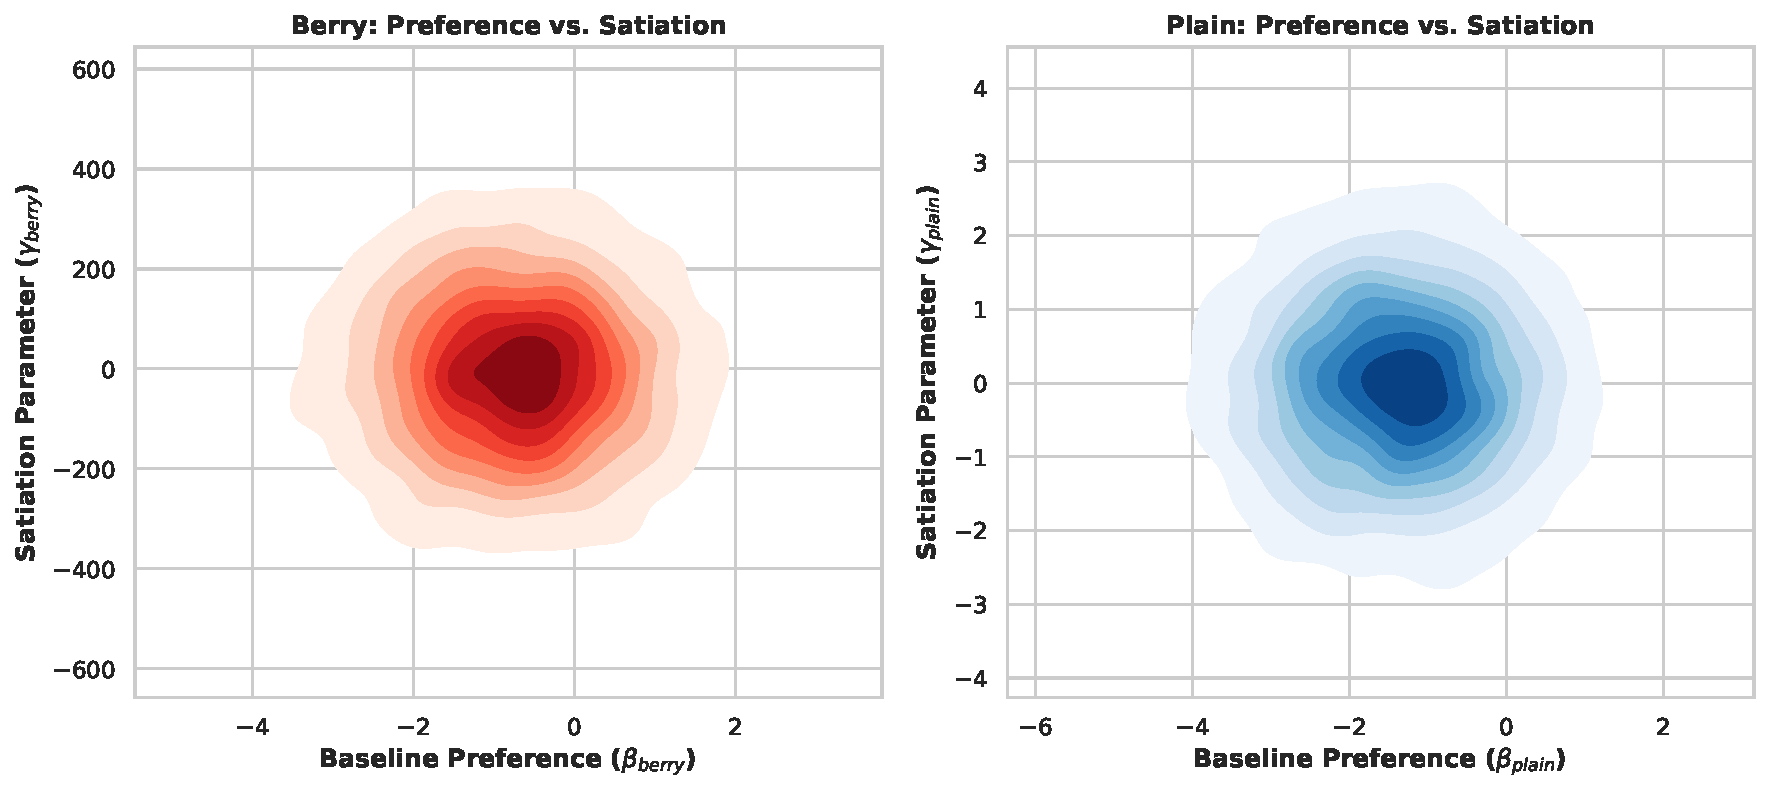
\includegraphics[height=.69\textheight,width=.95\textwidth,keepaspectratio]{fig5_joint_type_distributions.pdf}
\end{frame}
\begin{frame}[noframenumbering]{References}
\begin{itemize}
\item Attribute satiation: McAlister; Lattin (1987).
\item Variety and brand choice: Givon (1984); Chintagunta (1999).
\item Bundles and variety: Dub\'e (2004).
\item Price control functions: Petrin and Train (2010).
\item Personalized pricing: Dub\'e and Misra (2023).
\end{itemize}\small Full bibliographic entries appear in the accompanying paper.
\end{frame}
\end{document}
